\documentclass[runningheads]{llncs}

\usepackage[backend=biber]{biblatex}
\bibliography{AGI-book}

\usepackage[T1]{fontenc}
% T1 fonts will be used to generate the final print and online PDFs,
% so please use T1 fonts in your manuscript whenever possible.
% Other font encondings may result in incorrect characters.
%
\usepackage{graphicx}
% Used for displaying a sample figure. If possible, figure files should
% be included in EPS format.
%
% If you use the hyperref package, please uncomment the following two lines
% to display URLs in blue roman font according to Springer's eBook style:
%\usepackage{color}
%\renewcommand\UrlFont{\color{blue}\rmfamily}

\usepackage{amsmath}
\usepackage{amssymb}    % for \rightsquigarrow
\usepackage{wasysym}	% for frown face
% \usepackage{mathrsfs} % for \mathscr
\usepackage{eucal}	 	% for better-looking \mathcal
\usepackage{stmaryrd}
\usepackage{bm}
\usepackage{mathtools}		% to extend length of double harpoon arrows
\usepackage{tikz,ifthen}
\usetikzlibrary{arrows,positioning,decorations.markings,shapes.multipart,shapes.geometric,shapes.arrows,tikzmark,calc}
\usepackage{tikz-cd}
\usepackage{sidecap}
\usepackage{comment}
\usepackage{adjustbox}
\usepackage{hyperref}

\newcommand\logic[1]{{\color{gray}\mathsf{#1}}}
\newcommand*\sigmoid{\vcenter{\hbox{
\includegraphics{sigmoid.png}}}}

\makeatletter
\newcommand\mathcircled[1]{%
	\mathpalette\@mathcircled{#1}%
}
\newcommand\@mathcircled[3]{%
	\tikz[baseline=(math.base)] \node[draw,circle,inner sep=1pt] (math) {$\m@th#1#2$};%
}
\makeatother

\begin{document}
%
\title{Combining LLM, RL, and Logic}
%
%\titlerunning{Abbreviated paper title}
% If the paper title is too long for the running head, you can set
% an abbreviated paper title here
%
% \author{$\blacksquare\blacksquare\blacksquare\blacksquare$}
\author{King-Yin Yan \orcidID{0009-0007-8238-2442}}
%
% \authorrunning{$\blacksquare\blacksquare\blacksquare\blacksquare$}
\authorrunning{K-Y. Yan}
% First names are abbreviated in the running head.
% If there are more than two authors, 'et al.' is used.
%
% \institute{$\blacksquare\blacksquare\blacksquare\blacksquare$}
\institute{\email{general.intelligence@gmail.com}}
%
\maketitle              % typeset the header of the contribution
%
\begin{abstract}
This paper has two main ideas:  The first is to explain two types of LLM (large language model) + RL (reinforcement learning) architectures, which are probably known in ``folklore'' but not explicitly stated.  The second idea is based on what we call ``Type L'' architectures.  Under this perspective, formal logic is essentially the same as natural language, and so LLMs (language models) are the same as logic processors.  We briefly considered differentiable ``Logic Transformers'' but realized that current Transformers have very strong advantages over other alternatives.

\keywords{AGI \and large language models \and reinforcement learning \and neural-symbolic integration}
\end{abstract}

%\begin{tikzpicture}[remember picture,overlay]
%\node[draw, rectangle, red] at ([shift={(8cm,-2cm)}]current page.north west) {\huge\textbf{NOTE: unfinished draft}};
%\end{tikzpicture}

\section*{Part I. \ LLM + RL architectures}

For \textbf{string diagrams} \cite{Hinze2023} there are usually two conventions: 1) data are nodes, functions are edges: \tikz[baseline=(math.base)] \node[draw,circle,inner sep=1pt] (math) {$x$}; $\stackrel{f}{\longrightarrow}$ \tikz[baseline=(math.base)] \node[draw,circle,inner sep=1pt] (math) {$y$};  or alternatively 2) functions are nodes, data are edges: $\stackrel{x}{\longrightarrow}$ \tikz[baseline=(math.base)] \node[draw,circle,inner sep=1pt,fill=gray!20] (math) {$f$}; $\stackrel{y}{\longrightarrow}$.  In the following, I make explicit nodes for both functions (grey) and data (white), whereas edges merely represent linkages.

\begin{figure}
\label{fig:fundamental-forms}
\begin{tikzpicture}[every path/.style={thick},,decoration={
	markings,mark=at position 0.53 with {\arrow{>}}}]

\node[] (name) at (1.5,1.5) {\textbf{(RL)}};

\node[] (eye) at (-2, 0.25) {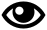
\includegraphics{eye-symbol.png}};
\node[] (mouth) at (-2, -0.25) {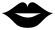
\includegraphics{mouth-symbol.png}};
\node[draw,thick,rectangle] (state) at (0, 0) {state $x$};
\node[draw,thick,circle,fill=gray!20] (RL) at (3.3, 0) {RL};
\node[draw,thick,cylinder,shape aspect=0.2,shape border rotate=90] (LTM) at (2.15,-0.1) {LTM};

\node[] (world) at (-1.3,1.3) {
\includegraphics[scale=0.6]{world-symbol.png}};
\node[rotate=-40] (approx) at (-0.6,0.7) {\LARGE$\approx$};

\draw[postaction={decorate},rounded corners=12pt] (state.north) to ([yshift=18pt]state.north) to ([yshift=12pt]RL.north) to (RL.north);
\draw[postaction={decorate},rounded corners=12pt] (RL.south) to ([yshift=-12pt]RL.south) to ([yshift=-18pt]state.south) to (state.south);

\draw[-left to,shorten >= 5pt] (eye) -- (state.north west);
\draw[-left to,shorten <= 5pt] (state.south west) -- (mouth);
% \draw[double=gray!20,double distance=3pt,implies-{implies[fill=gray!20]}] (state.east) -- (LTM);
\node[draw, double arrow, double arrow head extend=1.5pt, fill=gray!20, minimum height=26pt, inner ysep=1.6pt] at (1.15,0) {};
\end{tikzpicture}
\qquad
\begin{tikzpicture}[node distance=-2pt,every path/.style={thick},every text node part/.style={align=center},decoration={
	markings,mark=at position 0.53 with {\arrow{>}}}]

\node[] (name) at (0,1.5) {\textbf{(Auto-encoder / LLM)}};

\node[] (world1) at (-2,0) {
\includegraphics[scale=0.6]{world-symbol.png}};
\node[] (world2) at (2,0) {
\includegraphics[scale=0.6]{world-gray.png}};

\node[rotate=90,rectangle,fill=white] (state) at (0, 0) {state $x$};
\draw[] (state.south east) -- (state.north east) (state.south west) -- (state.north west);

\node (compress1) [rotate=90, draw, trapezium, trapezium angle=-70, fill=gray!20, minimum height=28pt, inner xsep=3.9pt, above=0pt of state] {};
\node (compress2) [rotate=90, draw,trapezium, trapezium angle=70, fill=gray!20, minimum height=28pt, inner xsep=3.9pt, below=0pt of state] {};

\node[] (rho) at (0.1,0) {\large $\rho \qquad \quad \; \rho^{-1}$};
%\node[] (rho-1) at (1,0) {$\rho^{-1}$};

\end{tikzpicture}
\caption{The eye represents observations and the mouth (speech) actions.  Because RL has to maximize rewards, its internal representation (the state) must eventually approach a good approximation of the world.  LTM = long term memory, which works by associative recall and condensation, but will not concern us in this paper.  The auto-encoder, of which LLMs are a special case, works by compressing world-data (via $\rho$) and de-compressing (via $\rho^{-1}$) to re-construct the data (grey world).}
\end{figure}

First let's recall the \textbf{fundamental forms} of RL (Fig.\ref{fig:fundamental-forms} left) and auto-encoders (right).  The question is how to combine them, for which we can ignore long-term memory (which we will eventually see, is just a very large Working Memory).  Both RL and LLM have the ``state'' $x$ in common but there are subtle differences as to how to interpret these states (Fig.\ref{fig:types-AB}).  Initially my research favored \textbf{Type W}, where the LLM is interpreted as a \textbf{world model}.  This approach suffers the problem that we don't really understand the internal state (marked ``?'') of LLMs, which consists of many layers of Transformers and their intermediate token outputs, so we don't know how to ``merge'' the RL state with the LLM state.

% 反省的有效性,取决于: 这个 loop 如何训练,有效地训练。

% (Other researchers have proposed different taxonomies \cite{?}).
It seems that \textbf{Type L} would be easier to work with, and it is also the ``mainstream'' approach, along the direction of RLHF \cite{Li2023}.  Here, the LLM simply loops over itself to complete the RL cycle.  LLM models the ``spoken thoughts'' of human thinking, as found in text corpora.  These thoughts are interpreted as internal states of the RL.  Ever since Richard Montague's success in converting a fragment of English into formal logic \cite{Montague1970} \cite{Montague1973}, the line between formal logic and natural language is blurred.  We should not obsess with the idea that ``logic'' must be some kind of cryptic, undecipherable code.  A new perspective is that \textit{the ``representation'' of human internal thought is just natural language} (or very close to it).

Type L also has the advantage that we can directly examine the internal state of an AGI.  What are currently called ``prompts'' is just \textbf{Working Memory}.  We can think of the prompt as something akin to our ``\textbf{inner speech}'' when thinking \cite{Haikonen2012}.

\begin{figure}
\label{fig:types-AB}
\begin{tikzpicture}[node distance=-2pt,every path/.style={thick},decoration={
	markings,mark=at position 0.53 with {\arrow{>}}}]

\node[rectangle, align=left, text depth=5pt, anchor=west, text width=100pt] at (-1.5, 2.25) {\textbf{(Type L)} LLM as \\ language model};

\node[draw,thick,dashed,rectangle, minimum height=66pt, rounded corners=10pt, minimum width=50pt, label=right:RL] (RL) at (2, 0) {};
\node (state) [draw,rectangle split,rectangle split parts=2,minimum width=3em] at (0, 0) {$x_{t}$ \nodepart{two} $x_{t+1}$};

\node[] (eye) at (-1.5, 0.27) {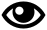
\includegraphics{eye-symbol.png}};
\node[] (mouth) at (-1.5, -0.27) {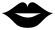
\includegraphics{mouth-symbol.png}};

\node[] (speech1) at (2,1.8) {
\includegraphics[scale=0.5]{speech-symbol.png}};
\node[] (speech2) at (2,-1.8) {
\includegraphics[scale=0.5]{speech-gray.png}};

\node (compress1) [draw,trapezium,trapezium angle=-70, fill=gray!20, minimum height=25pt, inner xsep=-6.5pt, anchor=south] at (2,0) {\footnotesize NL${}^{-1}$};
\node (compress2) [draw,trapezium,trapezium angle=70, fill=gray!20, minimum height=25pt, inner xsep=-2pt, below=0pt of compress1] {\footnotesize NL};

% \node (stateA) [rectangle,minimum width=35pt, minimum height=5pt, above=0pt of compress1] {};
% \draw(stateA.south west) -- (stateA.north west) -- (stateA.north east) -- (stateA.south east);
% \node (stateB) [rectangle,minimum width=35pt, minimum height=5pt, below=0pt of compress2] {};
% \draw(stateB.north west) -- (stateB.south west) -- (stateB.south east) -- (stateB.north east);

% \draw[dashed] (stateA.east) to ([yshift=-5pt]state.north west);
% \draw[dashed] (stateB.east) to ([yshift=5pt]state.south west);

\draw[-left to, shorten >= 3pt] (eye) -- ([yshift=7pt]state.west);
\draw[-left to, shorten <= 3pt] ([yshift=-7pt]state.west) -- (mouth);

\draw[postaction={decorate},rounded corners=12pt] (state.north) to ([yshift=27pt]state.north) to ([yshift=14pt]compress1.north) to (compress1.north);
\draw[postaction={decorate},rounded corners=12pt] (compress2.south) to ([yshift=-14pt]compress2.south) to ([yshift=-27pt]state.south) to (state.south);
\end{tikzpicture}
\qquad \quad
\begin{tikzpicture}[node distance=-2pt,every path/.style={thick},decoration={
	markings,mark=at position 0.53 with {\arrow{>}}}]

\node[align=left, anchor=west, text width=100pt] at (-1, 2) {\textbf{(Type W)} LLM as \\ world model};

\node[draw,thick,circle,fill=gray!20] (RL) at (1.5, 0) {RL};
\node (state) [draw,rectangle split,rectangle split parts=2,minimum width=3em] at (0, 0) {$x_{t}$ \nodepart{two} $x_{t+1}$};

\node[] (world1) at (-2,1.7) {
\includegraphics[scale=0.5]{world-symbol.png}};
\node[] (world2) at (-2,-1.7) {
\includegraphics[scale=0.5]{world-gray.png}};

\node (compress1) [draw,trapezium,trapezium angle=-70, fill=gray!20, minimum height=35pt, inner xsep=1pt, anchor=south] at (-2,0) {};
\node (compress2) [draw,trapezium,trapezium angle=70, fill=gray!20, minimum height=35pt, inner xsep=1pt, below=of compress1] {};

\node (stateA) [draw,trapezium,trapezium angle=-70, fill=white, minimum height=6pt, inner xsep=4pt, above=-22pt of compress1] {?};
\node (stateB) [draw,trapezium,trapezium angle=70, fill=white, minimum height=6pt, inner xsep=4pt, below=-22pt of compress2] {?};

\draw[dashed] (stateA.east) to [edge label=?] ([yshift=-5pt]state.north west);
\draw[dashed] (stateB.east) to [edge label'=?] ([yshift=5pt]state.south west);

\draw[postaction={decorate},rounded corners=12pt] (state.north) to ([yshift=14pt]state.north) to ([yshift=15pt]RL.north) to (RL.north);
\draw[postaction={decorate},rounded corners=12pt] (RL.south) to ([yshift=-15pt]RL.south) to ([yshift=-14pt]state.south) to (state.south);
\end{tikzpicture}
\caption{Two types of RL + LLM architectures. NL${}^{-1}$ is a map that compresses natural language to a hidden representation (not shown explicitly).}
\end{figure}

\textbf{The hallucination problem.}  The significance of combining RL and LLM is such that the system can \textit{think in loops}.  Reward maximization in the RL loop forces better thoughts to win, ie. those thoughts that are logically coherent with the rest of the learned knowledge.  This solves the problem of ``hallucinations'' when LLMs are just parroting human speech.  % This would   The remaining question is how to train the Type L model \textit{efficiently}, but this is more of an engineering rather than theoretical problem.

\section*{Part II. \ ``Logic''}

% ``Logic'' in quotes because, as I write this paper, I start to realize that neural associative memory (such as Transformer, which has been shown to be equivalent to Hopfield Networks \cite{Ramsauer2021}) may be a far superior form of ``logic'' than traditional, formal symbolic logic. % But I started this paper with differentiable symbolic logic, let's follow that idea.

As we know, LLMs predict the next word per each iteration.  % The number of possible natural-language sentences is an astronomical figure (if not $\infty$), so it is infeasible in practice to represent probability distributions over this set.  However, as vocabulary size is finite, the conditional probabilities $\mathbb{P}$(next word | prior words, context) are manageable.  % This part of LLMs efficiency -- by exploiting the decomposition of sentences into words.
%For a long time I tried to analyze the Transformer (Self Attention) from a symbolic-logic point of view, but did not know how to interpret the meaning of \textbf{tokens} -- do they correspond to logic propositions, or to sub-propositional symbols?  The question is how to reconcile these two views:
For a long time I have been trying to reconcile the following two views:
\begin{equation}
\nonumber
\hspace{-1cm} 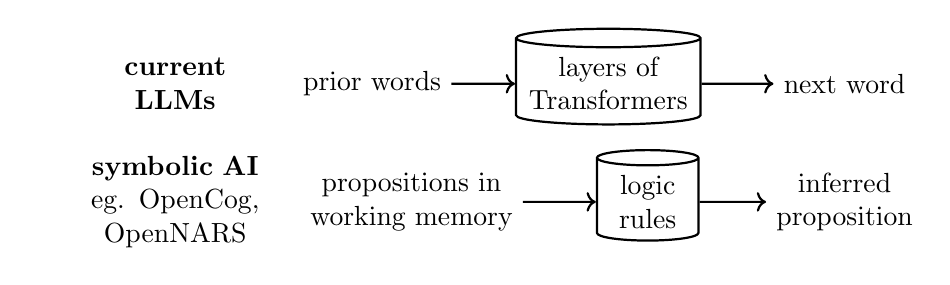
\begin{tikzpicture}[align=center, every path/.style={thick}]
\node[text width=100pt] at (-5.5, 0) {\textbf{current\\LLMs}};

\node (inputs1) [] at (-3,0) {prior words};
\node (KB1) [draw,thick,cylinder,shape aspect=0.1,shape border rotate=90,text width=60pt] at (0,0) {layers of\\Transformers};
\node (outputs1) [] at (3,0) {next word};

\draw[->] (inputs1) edge (KB1) (KB1) -- (outputs1);

% -------------------------------

\node[text width=100pt] at (-5.5, -1.5) {\textbf{symbolic AI}\\eg. OpenCog,\\OpenNARS};

\node (inputs2) [] at (-2.5,-1.5) {propositions in\\working memory};
\node (KB2) [draw,thick,cylinder,shape aspect=0.15,shape border rotate=90,text width=30pt] at (0.5,-1.5) {logic\\rules};
\node (outputs2) [] at (3,-1.5) {inferred\\proposition};

\draw[->] (inputs2) edge (KB2) (KB2) -- (outputs2);
\end{tikzpicture}
\end{equation}
until I had the insight that a logic-based system could output a proposition to rewrite part of a linguistic tree or graph, similar to the LLM outputting the next word to complete a sentence.

This leads us to the following basic architecture, which is also the setup proposed by Goertzel in \cite{Goertzel2021}:
\vspace{-0.5cm}
\begin{equation}
	\label{fig:KR-rewriting}
	\begin{tikzpicture}[baseline=(current bounding box.center), every path/.style={thick}]

		\node[rectangle, align=center, text depth=5pt, anchor=west, text width=100pt] at (-3.5, 0.2) {\small\textbf{KR\\structure}};

		\node[] at (-2.5, 0) {\Huge $\big($};
		\node[] (KR) at (0,0) {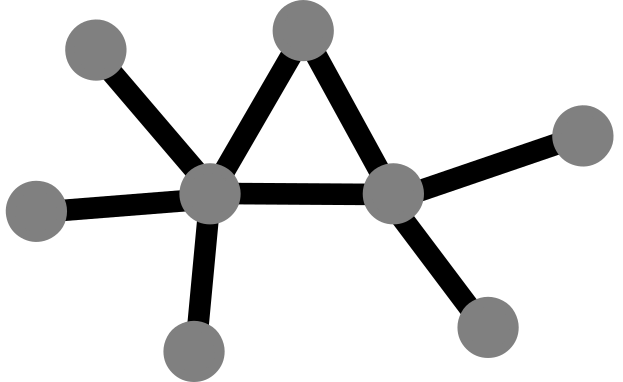
\includegraphics[scale=0.5]{KR-structure.png}};
		\node[] at (1, 0) {\Huge $\big)$};

		\node at (1.3,0) (here) {};
		\draw [->] (here) to[out=60, in=-60, looseness=10, "rewrite"] (here);
	\end{tikzpicture}
\end{equation}

One way to define a rewrite rule \cite{Kennaway1993} is as a pair of morphisms $L \leftarrow K \rightarrow R$, $L$ and $R$ are the left and right hand sides, and $K$ is the interface graph.  $G$ is the input graph and $H$ is the result of rewriting.  The effect is that the part of $L$ outside $K$ is deleted from $G$ and is replaced by the part of $R$ outside $K$:
\begin{equation}
	\label{eqn:rewrite-rule}
	\begin{tikzcd}
		L \arrow[d] & K \arrow[l] \arrow[d] \arrow[r] & R \arrow[d] \\
		G & D \arrow[l] \arrow[r] & H
	\end{tikzcd}
\end{equation}
This occurs in a category where graphs are objects and homomorphisms define some notion of ``matching''.  Now if we imagine a \textbf{differentiable} version of rewriting rules (see (\ref{eqn:differentiable-variable-slots}) below \footnote{with experimental code available on \href{https://github.com/Cybernetic1/reinforcement-learning-experiments}{https://github.com/Cybernetic1/reinforcement-learning-experiments}}), all the rules would be represented by a set of parameters $\Theta \in \mathbb{R}^n$, and the parameterized rules \textit{must} cover the entire family of rewrite rules as $\Theta$ vary continuously (in practice, we can limit the rules length to make that possible).  This requires the use of ``\textbf{discretizing}'' functions such as sigmoid and softmax, and may be formulated by a fairly mechanical process.  However, in doing so we have overlooked the possibility that a \textbf{deep} neural network such as Transformer may be able to aggregate all the contents of Working Memory, output some intermediate \textbf{distributive} representations, before finally outputting some discrete tokens.  Such a process would imply $L$ matches the entire input graph $G$ in (\ref{eqn:rewrite-rule}).

% Finally I had a break-through insight that a symbolic-logic Transformer should output \textbf{atomic propositions} that modify a linguistic tree \textbf{at one position} at a time (Fig.\ref{fig:flat-vs-tree}).  Tree structure simplifies the implementation of logic rules -- fewer parameters needed; learns faster.  An analogy is that humans try to parse sentences syntactically first (which requires only superficial information such as parts-of-speech) before deeper semantic understanding.  In order words, grammar \textit{simplifies} subsequent understanding.

%\begin{figure}
%% NOTE: use ~/Downloads/GraphML-to-Tikz to convert graphML to Tikz, then edit Tikz
%\centering
%\begin{tikzpicture}[every path/.style={thick}]
%\begin{scope}[scale=2.5]
%\tikzstyle{defnode}=[draw,rectangle,rounded corners=4pt,node font=\small,inner ysep=1pt]
%
%\node (a) [defnode] at (-1, 0)   {I\strut};
%\node (b) [defnode] at (-0.5, 0) {love\strut};
%\node (c) [defnode] at (0, 0)    {you\strut};
%\node (d) [defnode] at (0.5, 0)  {to\strut};
%\node (e) [defnode] at (1, 0)    {pieces\strut};
%
%\foreach \n/\m in {a/b,a/c,a/d,a/e,b/c,b/d,b/e,c/d,c/e,d/e} {
%	\draw (\n.north) to[bend left] node[above] {} (\m.north); }
%\end{scope}
%\begin{scope}[shift={(5.5,0.2)},scale=1.5,rotate=-20]
%\tikzstyle{defnode}=[draw,rectangle,rounded corners=4,thick,node font=\small]
%\tikzstyle{defedge}=[->,thick]
%
%\node(I) at (-1,0)       [defnode] {I};
%\node(love) at (0,0)     [defnode] {love};
%\node(you) at (1,0)      [defnode] {you};
%\node(to) at (0,0.6)     [defnode,gray] {to};
%\node(pieces) at (1,0.6) [defnode,gray] {pieces};
%
%\draw[defedge](I) edge (love) (love) edge (you);
%\draw[defedge,gray] (to) edge (love) (to) edge (pieces);
%\end{scope}
%\end{tikzpicture}
%\caption{\textbf{Left:} In traditional Self-Attention Transformer, each token is related to every other token, ie. fully connected graph.  \textbf{Right:}  Example of a linguistic tree or graph, where only some nodes are connected.  From a \textbf{Chomskyan} perspective, any NL sentence can fit into a tree structure.  This example starts with a simple relation, I-love-you, and the ``love'' node is modified by a ``to'' clause (grey).  Let's not dwell too deep into this example, as machine-learning will fill in such details.}
%\label{fig:flat-vs-tree}
%\end{figure}

% Having convinced ourselves that LLMs can be a model of \textit{internal} thoughts, we wonder if the Transformer can be re-formulated as some kind of logic engine or general \textbf{rewriting system}, defined by rewriting \textbf{rules} that can be learned via gradient descent?

% \textbf{Knowledge Representation}. We may endow the KR structure with additional structures such as:  1) tree structure as inspired by Chomskyan linguistics; 2) ontology encoded as topological ordering (eg. ``cones'') in vector space; 3) probabilistic or fuzzy strength as the size of a thought vector.  This implies that thoughts are directions on a hypersphere, as some researchers have noted of Transformer tokens \cite{Pochinkov2023}.

% \textbf{Graph-rewriting}.  In \cite{Goertzel2021} \cite{Goertzel2021b}, Goertzel formulates intelligence as the re-writing of some metagraph or hypergraph structure, which is essentially the same as the author's idea of tree as Working Memory and which I now link to the Transformer.  Rewriting is defined categorically as certain morphisms, requiring some diagrams to commute.  This defines intelligence in \textbf{algebraic} terms, and it requires the discretizing functions above to achieve such algebraic rewriting.

% \textbf{The Rete algorithm} is another classical AI technique to accelerate rules-matching.  It is based on the observation that Working Memory changes incrementally, so one should find matchings from the ``delta'' change instead of the entire memory content.  In a sense we are re-tracing many classical AI ideas and adapting them to the new LLM setting.  In this case, we can learn a probabilistic function from Working Memory to rules which are most likely applicable.  This increases efficiency while still maintaining differentiability.

%{\color{red} Update:  need to handle \textbf{variable-length propositions}.  Need tree-rewriting logic.  In a certain direction, the neural network may end up with a form very close to or even identical to current Transformers.}
%\begin{equation}
%	\nonumber
%	\vcenter{\hbox{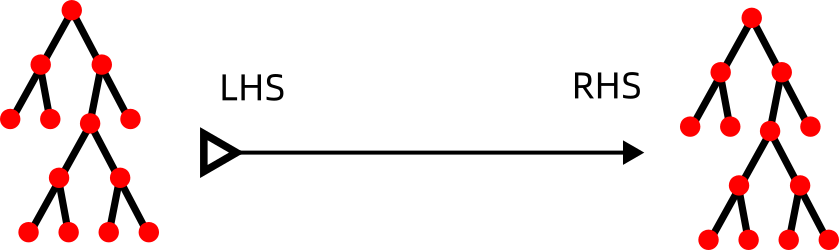
\includegraphics[scale=0.7]{tree-rewriting.png}}}
%\end{equation}

% Now we are ready to re-formulate the Transformer as applying a set of logic / symbolic rules to its inputs.  In order for such rules to be \textbf{differentiable}, we can't have $N$ rules at one moment and then suddenly $N+1$ rules the next moment (that would not be differentiable).  The only solution I can think of is to maintain a \textit{fixed} number, $M$, of rules.  Every rule may potentially ``morph'' into any other rule in this space of rules.  The set of rules would look like a \textit{rectangular} matrix: {\color{red}(This part needs modification for tree-based logic rules instead of fixed-length rules; Tree-based rules require special syntax.  This may not be too difficult, as tree-rewriting is equivalent to term-rewriting, which the author already has some familiarity with.  [Goertzel 2021] also developed a ``reflective metagraph rewriting as a foundation for an AGI language of thought'')}

%\begin{equation}
%\begin{aligned}
%\mbox{rule 1:} & \quad \boxed{X^1_{11}... X^1_{1I}} \;\wedge\; \boxed{X^1_{21} ... X^1_{2I}} \;\wedge\;...\; \boxed{X^1_{K1} ... X^1_{KI}} \rightarrow \boxed{X^1_{01} ... X^1_{0I}} \\
%\mbox{rule 2:} & \quad \boxed{X^2_{11}... X^2_{1I}} \;\wedge\; \boxed{X^2_{21} ... X^2_{2I}} \;\wedge\;...\; \boxed{X^2_{K1} ... X^2_{KI}} \rightarrow \boxed{X^2_{01} ... X^2_{0I}} \\
%.... & \quad .... \\
%\mbox{rule M:} & \quad \boxed{X^M_{11}... X^M_{1I}} \;\wedge\; \boxed{X^M_{21} ... X^M_{2I}} \;\wedge\;...\; \boxed{X^M_{K1} ... X^M_{KI}} \rightarrow \boxed{X^M_{01} ... X^M_{0I}}
%\end{aligned}
%\end{equation}

%For a rule to be applicable, its atoms must match with propositions in Working Memory.  An atom may contain constants (such as ``Socrates'', that must be matched correspondingly) or variables (such as $x$, that matches any entity).  To achieve this, I introduce a trick called \textbf{cylindrification factor} (Fig.\ref{fig:cylindrify-example}).

%\begin{figure}
%	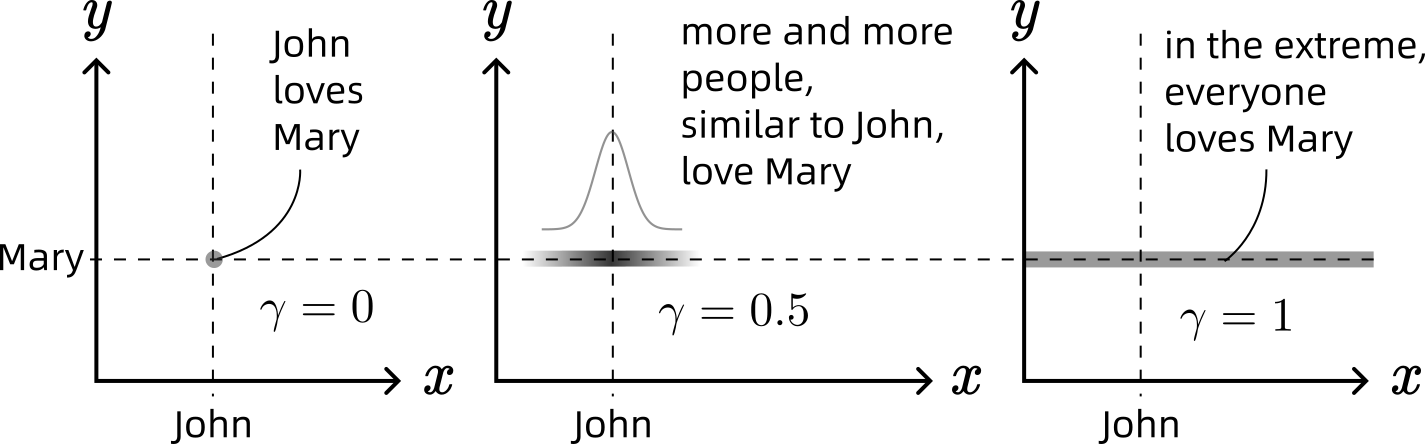
\includegraphics[scale=.6]{cylindrify-example.png}
%	\caption{Illustration of the cylindrification factor $\gamma$.}
%	\label{fig:cylindrify-example}
%\end{figure}

%\begin{equation}
%	\gamma =\begin{cases}
%		\approx 0 \Rightarrow \mbox{constant, do matching, TV = match degree} \cdot \sigmoid(1 - \gamma) \\
%		\approx 1 \Rightarrow \mbox{variable, do substitution, TV = 1} \cdot \sigmoid(\gamma)
%	\end{cases}
%\end{equation}
%Each position inside a rule can be either a constant or variable, and their treatments are obviously very different, but the results of the two streams would be super-imposed (added) together, pretty much like the \textbf{superposition} of quantum states.

%To make \textbf{variable substitution} differentiable is even trickier.  Consider this logic rule:
%\begin{equation}
%\logic{father}(X_1,X_2) \wedge \logic{father}(X_2,X_3) \rightarrow \logic{grand\hbox{-}father}(X_1,X_3)
%\end{equation}

%We have to imagine some ``slots'' where we ``select'' variables using weights and \textbf{softmax}:
%\vspace{-0.2cm} \begin{equation}
%\logic{father}(
\begin{tikzpicture} \draw[line width=3pt, gray!50] (0.2,0.9) -- (0.2,0) (0.5,0.9) -- (0.5,0) (0.8,0.2) -- (0.8,0); \draw[thick] (0,0) to (1,0); \end{tikzpicture})
%\wedge
%\logic{father}(
\begin{tikzpicture} \draw[line width=3pt, gray!50] (0.2,0.2) -- (0.2,0) (0.5,0.9) -- (0.5,0) (0.8,0.9) -- (0.8,0); \draw[thick] (0,0) to (1,0); \end{tikzpicture})
%\rightarrow
%\logic{grand\hbox{-}father}(
\begin{tikzpicture} \draw[line width=3pt, gray!50] (0.2,0.9) -- (0.2,0) (0.5,0.2) -- (0.5,0) (0.8,0.9) -- (0.8,0); \draw[thick] (0,0) to (1,0); \end{tikzpicture})
%\end{equation}

%\textbf{Differentiable symbolic logic}.  In order to implement differentiable logic rules, I came up with a mechanism sort of like ``loading'' and ``unloading'' tokens into variable slots:
Part of a differentiable rewriting rule may look like this:
\begin{align}
\nonumber
& \qquad \qquad \tikzmark{Y1}
\setlength{\fboxrule}{3pt}
\fcolorbox{gray!50}{white}{$\hat{x}^1$}
\qquad
\tikzmark{Y2} \fcolorbox{gray!50}{white}{$\hat{x}^2$}
\qquad
\tikzmark{Y3} \fcolorbox{gray!50}{white}{$\hat{x}^3$} \\
\label{eqn:differentiable-variable-slots}
& \qquad w_{ij}^k \\
& \nonumber \\
& \logic{father}(\tikzmark{X11} x_{11}, \tikzmark{X12} x_{12}, \tikzmark{X13} \bullet_{13}) \wedge
\logic{father}(\tikzmark{X21} \bullet_{21}, \tikzmark{X22} x_{22}, \tikzmark{X23} x_{23}) \rightarrow \logic{grand\hbox{-}father}(x_1,\bullet_2,x_3)
\nonumber

\begin{tikzpicture}[remember picture,overlay]
\draw (pic cs:Y1) +(10pt,-7pt) -- ($ (pic cs:X11) +(7pt,12pt) $);
\draw (pic cs:Y1) +(10pt,-7pt) -- ($ (pic cs:X12) +(7pt,12pt) $);
\draw (pic cs:Y1) +(10pt,-7pt) -- ($ (pic cs:X13) +(7pt,12pt) $);
\draw (pic cs:Y1) +(10pt,-7pt) -- ($ (pic cs:X21) +(7pt,12pt) $);
\draw (pic cs:Y1) +(10pt,-7pt) -- ($ (pic cs:X22) +(7pt,12pt) $);
\draw (pic cs:Y1) +(10pt,-7pt) -- ($ (pic cs:X23) +(7pt,12pt) $);
\draw (pic cs:Y2) +(10pt,-7pt) -- ($ (pic cs:X11) +(7pt,12pt) $);
\draw (pic cs:Y2) +(10pt,-7pt) -- ($ (pic cs:X12) +(7pt,12pt) $);
\draw (pic cs:Y2) +(10pt,-7pt) -- ($ (pic cs:X13) +(7pt,12pt) $);
\draw (pic cs:Y2) +(10pt,-7pt) -- ($ (pic cs:X21) +(7pt,12pt) $);
\draw (pic cs:Y2) +(10pt,-7pt) -- ($ (pic cs:X22) +(7pt,12pt) $);
\draw (pic cs:Y2) +(10pt,-7pt) -- ($ (pic cs:X23) +(7pt,12pt) $);
\draw (pic cs:Y3) +(10pt,-7pt) -- ($ (pic cs:X11) +(7pt,12pt) $);
\draw (pic cs:Y3) +(10pt,-7pt) -- ($ (pic cs:X12) +(7pt,12pt) $);
\draw (pic cs:Y3) +(10pt,-7pt) -- ($ (pic cs:X13) +(7pt,12pt) $);
\draw (pic cs:Y3) +(10pt,-7pt) -- ($ (pic cs:X21) +(7pt,12pt) $);
\draw (pic cs:Y3) +(10pt,-7pt) -- ($ (pic cs:X22) +(7pt,12pt) $);
\draw (pic cs:Y3) +(10pt,-7pt) -- ($ (pic cs:X23) +(7pt,12pt) $);
\end{tikzpicture}
\end{align}
%\begin{equation}
%\hat{x}^k \mathrel{:}= \underset{\text{predicates}}{\forall i \in} \; \underset{\text{arguments}}{\forall j \in} \left\langle \mathrm{soft}\max_{ij} w_{ij}^k \; , \; x_{ij} \right\rangle
%\end{equation}
which has a form quite similar to the \textbf{Self-Attention} of Transformers (right):
%\begin{equation}
%\text{Attention}(\mathbf{Q,K,V}) = \text{soft}\max  \frac{\langle \mathbf{Q,K} \rangle}{\sqrt{d_k}} \mathbf{V}
%\end{equation}
\begin{equation}
	\vcenter{\hbox{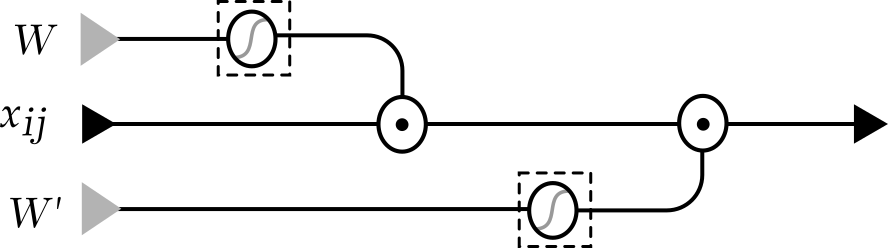
\includegraphics[scale=0.4]{logic-Transformer-string-diagram.png}}}
	\quad
	\vcenter{\hbox{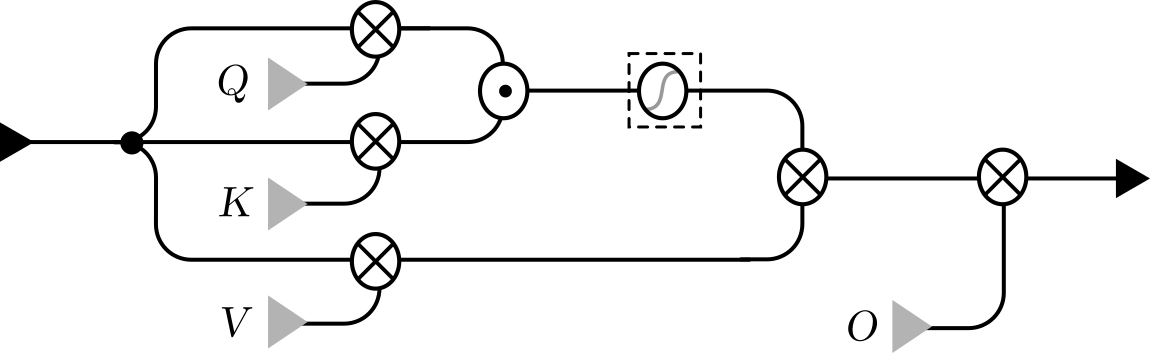
\includegraphics[scale=0.4]{Attention-string-diagram.png}}}
\end{equation}
but the rule (\ref{eqn:differentiable-variable-slots}) neglected the fact that the variables in each $\mathsf{father}$ atom must match their variables with each other (a situation well-known in classical logic-based AI).  This means we have to programmatically feed all \textit{pairs} of Working-Memory atoms, ie. the Cartesian product $A \times A$, into the above string diagram.  That makes it different from the Transformer which takes its input in plain form.  The reason why Transformer can do that is because it has many \textbf{layers}, and the matching of $A \times A$ can be achieved over these layers.

% except that softmax does not commute with inner products, so they are not exactly equivalent, but qualitatively similar.
Indeed, neural \textbf{associative memory} (such as Transformer, which are shown to be equivalent to Hopfield Networks \cite{Ramsauer2021}) may be a far superior form of ``logic'' than traditional, formal symbolic logic.  Consider the logic example:
\begin{equation}
	\mbox{loves}(X, Y) \wedge \neg \mbox{loves}(Y,X) \rightarrow \frownie(X)
\end{equation}
but we immediately sense that the human brain does not work like that.  It is more like: the thought of unrequited love fires a massive number of neural activations which all point to the conclusion that this is an unhappy experience.  The Transformer's associative memory does exactly that.

% Let's pause for a moment to reflect that we tried to substitute variables (some kind of syntactic manipulation), and ended up with something like Self-Attention.
Also recall that Self-Attention originated as a kind of \textbf{content-addressable memory} for Neural Turing Machines, invented for its differentiability.  In retrospect, it is also a very efficient implementation of associative memory.  If we want to improve the Transformer, we should first understand it as an associative memory.

% \textbf{Relation algebra}.  The matching of terms containing variables is combinatorially expensive - a fact well-known to an older generation of AI researchers.  To get around this problem, perhaps we can turn to relation algebra which has long established as a variable-free formalism.  For example, ``father's father is grandfather'' ($F; F = G$) is very close to human thinking.  I propose to extend beyond relations in the traditional sense, to a graphical knowledge representation where edges are ``linguistic'' relations.  For example: ``love and not loved back implies heartbreak'' ($\heartsuit ; \overline{\heartsuit}^\top \vdash \frownie$) does not mean that $\frownie$ is a relation with oneself; rather it is an inferred attribute, or unary predicate.  This example shows that the general rule about heartbreaks is independent of the individuals involved, as it should, and it has a form highly similar to relation algebra.  Inspired by Tarski's view that relation algebra can express most of mathematics\cite{Maddux2006} \cite{Schmidt2010}, we have grounds to believe that rewriting rules matching over linguistic graphs with labeled edges is plausibly powerful enough to express all of human intelligence.

% A final obstacle concerns the limitations of first-order logic.  As Ben Goertzel pointed out during an online discussion, my earlier design lacked mechanisms for handling \textbf{Skolem functions} and thus existential quantifiers.  One way to get around this problem is to define $\exists$ via a set of \textbf{higher-order logic} rules.  Without explicitly specifying how to do so (though I believe this can be done), we simply use a more powerful ``higher-order'' logic in the sense that rules admit substitutions in all (predicate or argument) positions, and hope that machine learning will learn the required axioms.

% Armed with these ideas, it is not too difficult to work out a new kind of differentiable ``Logic Transformer'' (Fig.\ref{fig:string-diagram}).  A detailed explanation is contained in my on-going research thesis \cite{YKY}.

%\begin{figure}
%	\hspace{-3cm}
%	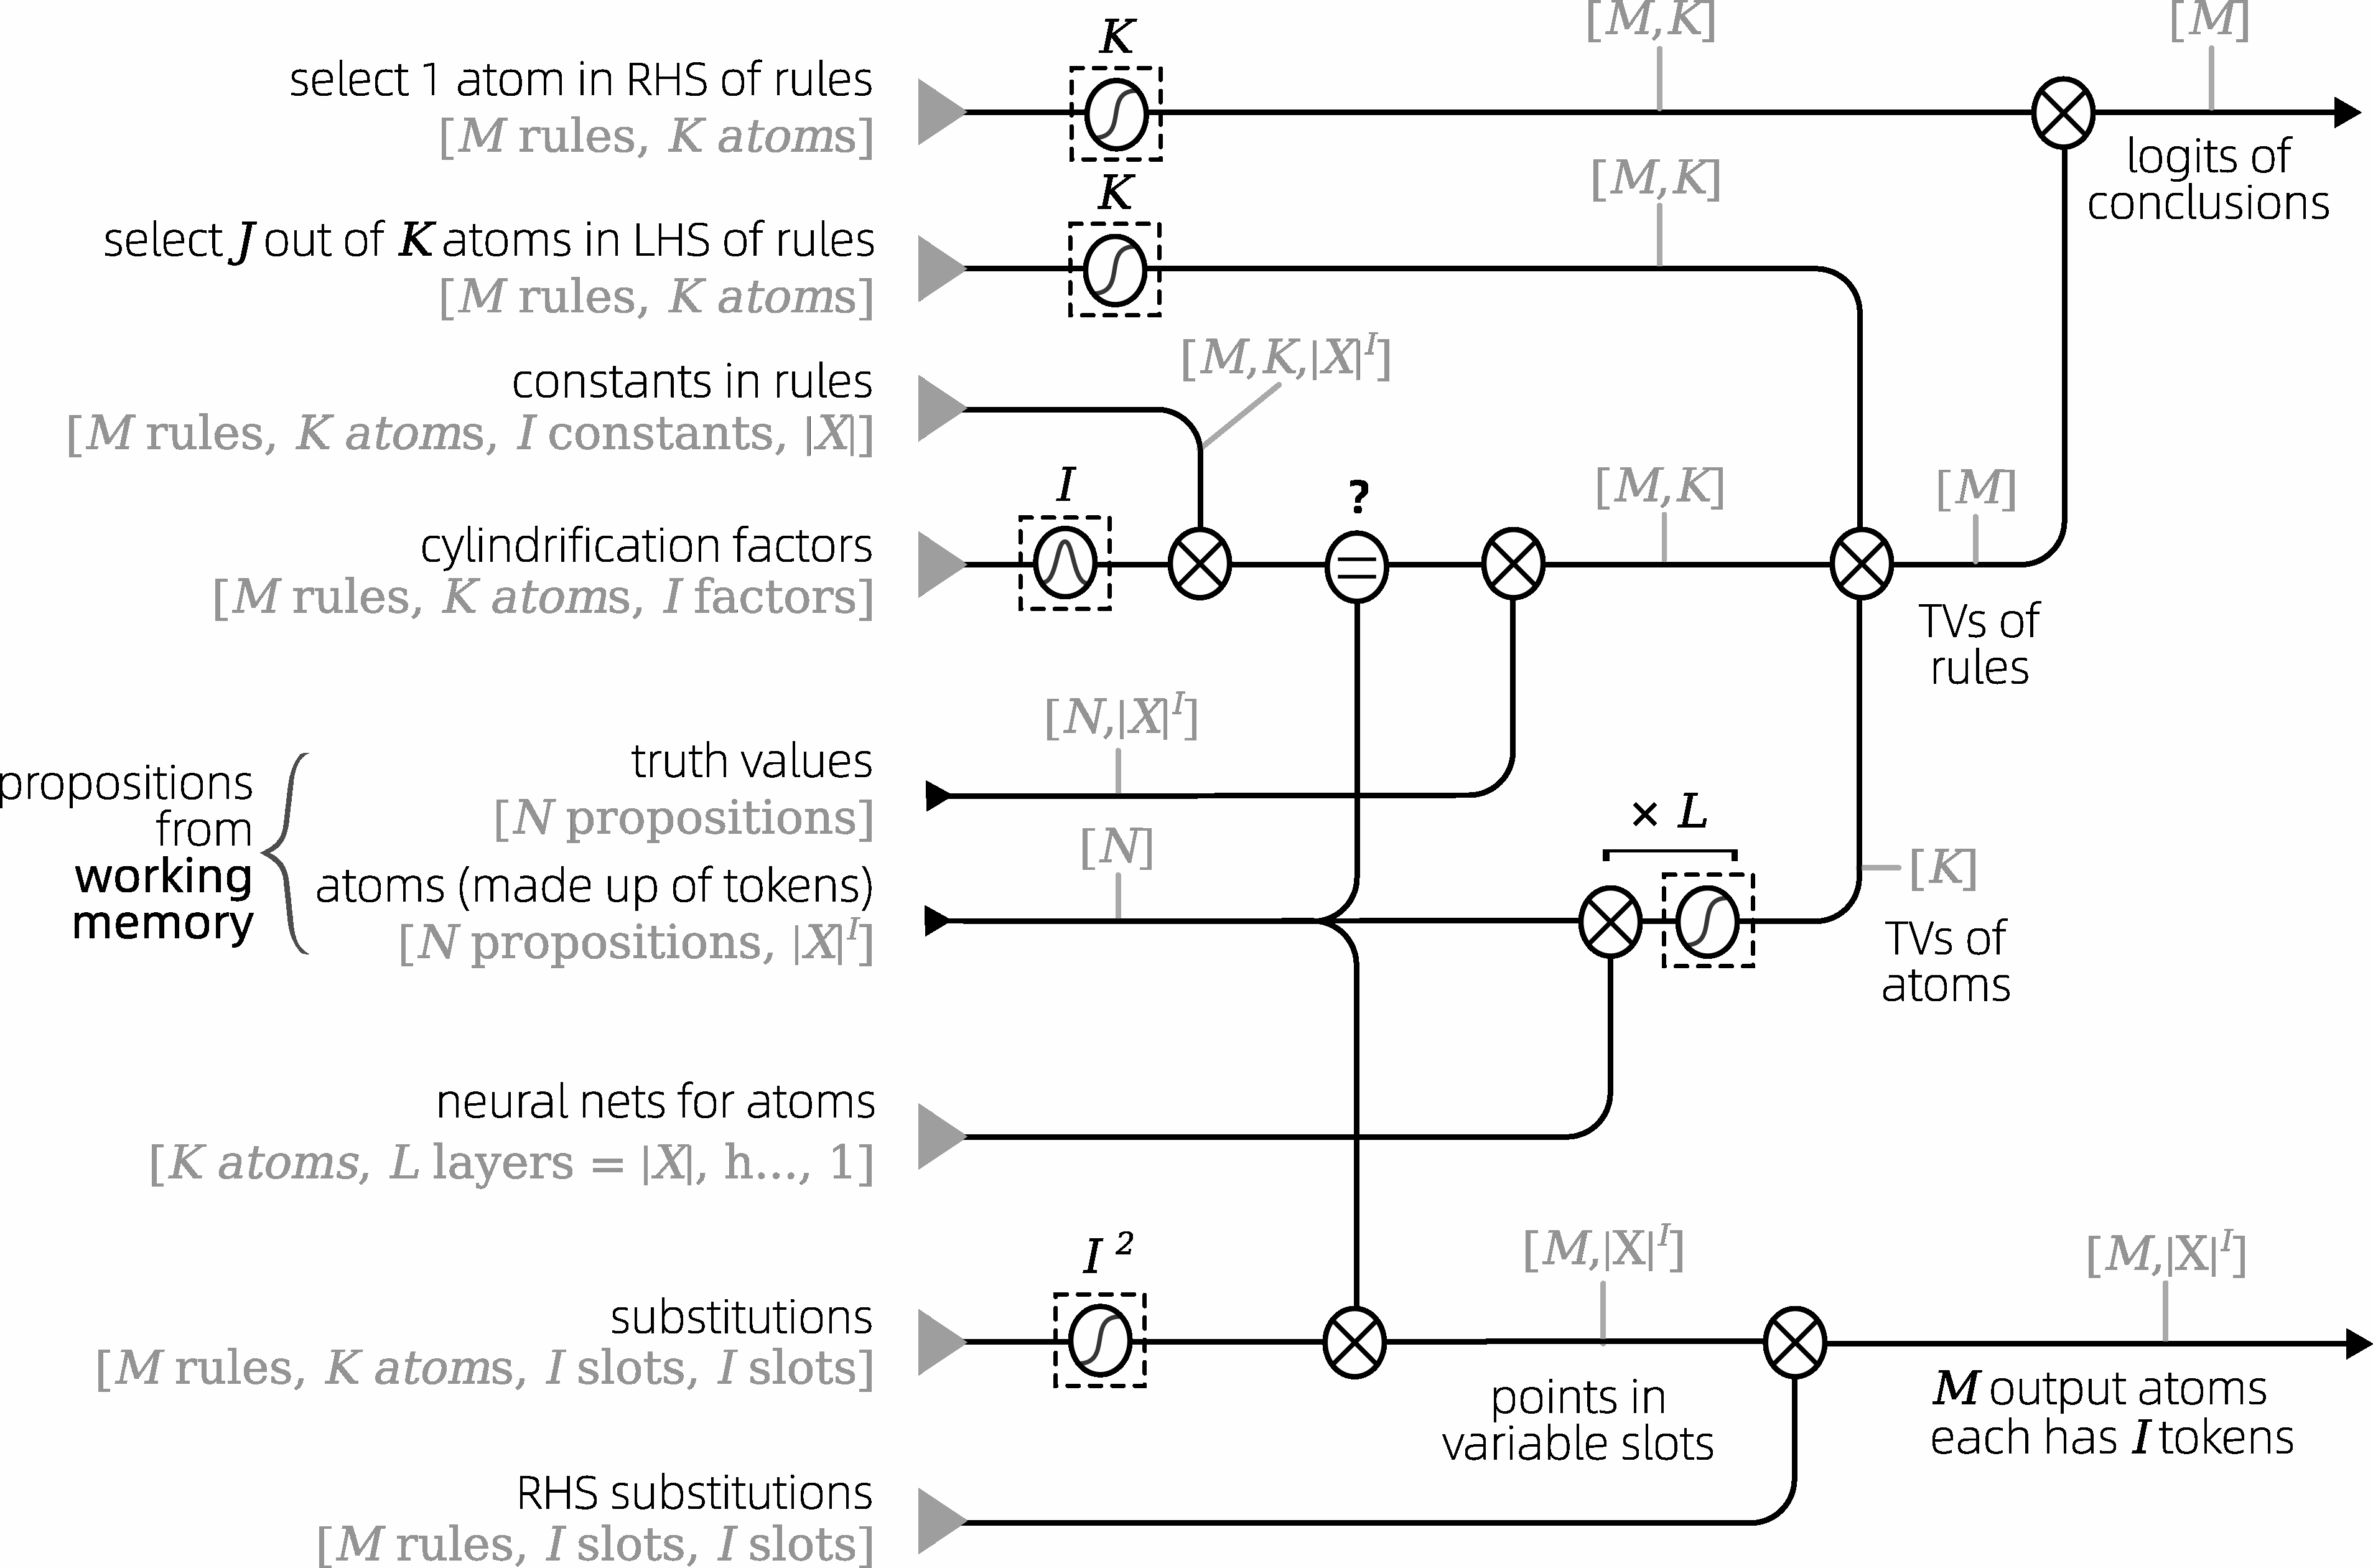
\includegraphics[scale=.7]{logic-Transformer-string-diagram-3.png}
%	\caption{String diagram of the Logic Transformer.  The {\LARGE\color{gray}\RIGHTarrow} indicates \textbf{internal data} supplied by the Transformer, similar to the Q,K,V matrices in traditional Transformers.  These are modified through ``learning'' or training.  The 2 \RIGHTarrow's \ are \textbf{inputs} to the Transformer, this is matched with the 2 \textbf{outputs} on the right of the diagram.  Tags {\color{gray}$[M,N,...]$} indicate the \textbf{dimensions} of data streams.  {\color{red}NOTE:  diagram is obsolete as it pertains only to fixed-length propositions.}}
%	\label{fig:string-diagram}
%\end{figure}
%

% I guess I am not the only one among AGI researchers who is jealous of the success of the Self-Attention Transformer BERT-GPT lineage tradition.  Many like us suspect that Transformers are unnecessarily ``bulky'', meaning that they can be reduced or simplified.  But how?

% Functor $\mathsf{F}: \mathcal{C} \rightarrow \mathcal{D}$.
From a \textbf{functorial} point of view (eg.\cite{Crescenzi2024} \cite{Abbott2024} \cite{Khatri2024}), one can find a functor that transforms a category $\mathcal{C}$ of KR structure and rewrite morphisms into another category $\mathcal{D}$ with different KR structure and rewrite morphisms.  It might just happen that one type of rewrite morphisms are computationally less costly than the other type, and so we have discovered a better, more efficient AGI system.  But this maneuver seems not so useful in light of the fact that Transformer / Self Attention is a distributive associative memory that may not care too much about its input representation.

% String diagrams allow us to visually compare architectures, such as Self-Attention with my differentiable Logic Transformer.  These diagrams can be ``morphed'' by rewriting rules.  One research team proposed universal approximators as an equivalence class of architectures under rewriting, but such a class is too permissive and pretty useless.  We want a more refined view of architectures such that we can distinguish which ones are more \textbf{learning-efficient} -- the key question in AGI development.

% If all continuous functions are equivalent, then what sets them apart?  My idea is that functions such as sigmoid and softmax are ``tearing'' the input space irreversibly, due to finite precision, into \textbf{discrete} regions that are no longer connected.  This process is crucial to eg. Transformer's ability to output discrete tokens.

% In Ben Goertzel's ``General Theory of General Intelligence'', he formulates intelligence as the re-writing of some metagraph or hypergraph structure, which is essentially the same as my idea of tree as Working Memory and which I now link to the Transformer.  Rewriting is defined categorically as certain morphisms, requiring some diagrams to commute.  This defines intelligence in \textbf{algebraic} terms, and it requires the discretizing functions above to achieve such algebraic rewriting.

% But the Transformer has also been shown capable of discrete (syntactic) manipulations.  Does that mean that all functions with discretizing ability are equivalent?  Can the Transformer be replaced by a fully-connected NN with sigmoid activation?  Seems unlikely, and if not, then what sets them apart \textit{still}?  Well, an obvious answer is that we need to \textbf{count computations}.

\section*{Conclusion}

We proposed a simple AGI architecture that looks promising.  If the Transformer cannot be improved much further, we should perhaps accept the current design and proceed to the ``engineering'' phase of AGI development.

\printbibliography

\end{document}
